\documentclass{article}
\setlength{\parskip}{5pt} % esp. entre parrafos
\setlength{\parindent}{0pt} % esp. al inicio de un parrafo
\usepackage{amsmath} % mates
\usepackage[sort&compress,numbers]{natbib} % referencias
\usepackage{url} % que las URLs se vean lindos
\usepackage[top=25mm,left=20mm,right=20mm,bottom=25mm]{geometry} % margenes
\usepackage{hyperref} % ligas de URLs
\usepackage{graphicx} % poner figuras
\usepackage[spanish]{babel} % otros idiomas
\usepackage[utf8]{inputenc} % alparecer son los acentos
\documentclass[12pt,letterpaper]{article}
\usepackage[utf8]{inputenc}
\usepackage{tikz}
\usetikzlibrary{trees}
\usepackage[spanish, es-nodecimaldot]{babel}
\usepackage{color}
\usepackage{algorithm}
\usepackage[noend]{algpseudocode}
\renewcommand{\algorithmicrequire}{\textbf{Entrada:}}
\renewcommand{\algorithmicensure}{\textbf{Salida:}}
\usepackage{subcaption}
\usepackage{amsfonts}
\usepackage{hyperref}
 \hypersetup{
     colorlinks=true,
     linkcolor=blue,
     filecolor=blue,
     citecolor = blue,      
     urlcolor=cyan,
     }
\usepackage{amssymb}
\usepackage{listings}
\usepackage{color}
\author{I E G} % author
\title{Práctica 7 : Búsqueda local} % titulo
\date{\today}

\begin{document} % inicia contenido

\maketitle % cabecera

\begin{abstract} % resumen
Lo que nos interesa hacer es encontrar puntos máximos de funciones para este caso particular buscando el máximo de una función, es decir, maximizar \cite{elis7} alguna variante de la función bidimensional $(x,y)$, con restricciones $g−3\leq x,y \leq 3$, en donde la posición actual es un par $(x,y)$ en donde se requieren dos movimientos aleatorios en $\Delta x$ y $\Delta y$, cuya combinación genera ocho posibles vecinos figura \ref{figura1}, de los cuales se selecciona el que obtiene el mayor valor para $g(x,y)$, y crear, posteriormente, una animación de las réplicas simultáneas de la búsqueda local.

La función utilizada para esta práctica es:

\begin{align*}
g(x,y) &= \frac{((x + 0.7)^4 - 50 * x^2 - 50 * x + (y + 0.7)^4 - 50 * y^2 + 50 * y)}{300}.
\end{align*}

\begin{figure} [h!]% figura
    \centering
    \includegraphics[width=129mm]{Figura1.png} % archivo
    \caption{Función tridimencional $g(x,y)$.}
    \label{figura1}
\end{figure}

\end{abstract}


\section{Desarrollo}

La función tiene varios valles con mínimos valores locales y mayores locales, en la función pondremos pseudoaliatoriamente valores de $x$ y de $y$ y de esta forma hacer la búsqueda local con varios puntos de color rojo con la justificación es de no atascarse en mínimos globales mientras el punto verde es la posición deseada de búsqueda local.
En este caso se considera \cite{fab} la la función $g(x,y) | −3 \leq x,y \leq 3$ el método utilizado \cite{denis} para maximizar la función, tiene que consistir en el posicionamiento de los puntos $(x,y)$ en el plano y dados $\Delta x$ y un $\Delta y$ se consideran ocho vecinos de modo que los puntos rojos van buscando la mejor posición de forma automatizada como en la \href{https://github.com/IsaacEstrada159/simulacion/blob/master/p7/images/5/ezgif.com-gif-maker%20(11).gif}{animación}.

\section{Experimento}

En esta sección se demuestra en la figura \ref{graficas} de los diferentes experimentos variando los pasos.

\begin{figure} [h!]
 	\centering
 	\begin{subfigure}[b]{0.40\linewidth}
 		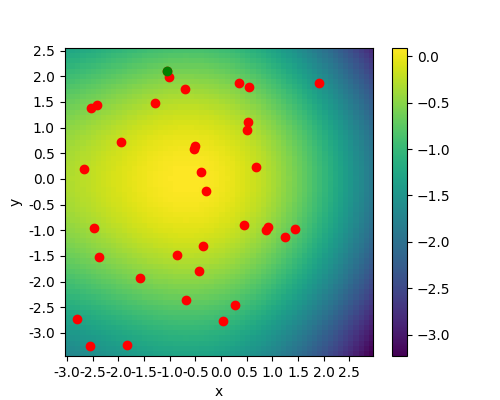
\includegraphics[width=\linewidth]{p7_v_t01.png}
 		 \caption{Paso 1 de $g(x,y)$.}
 		\label{3d}
 	\end{subfigure}
 	\begin{subfigure}[b]{0.40\linewidth}
 		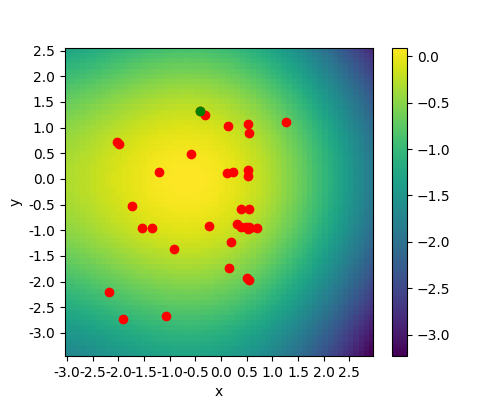
\includegraphics[width=\linewidth]{p7_v_t08.png}
 		 \caption{Paso 3 de $g(x,y)$.}
 		\label{levelplot}
 	\end{subfigure}
 	 	\begin{subfigure}[b]{0.40\linewidth}
 		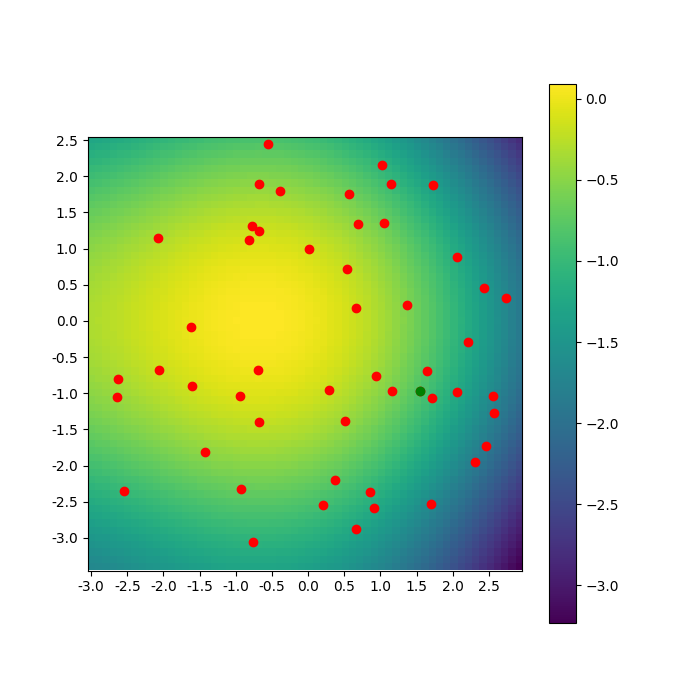
\includegraphics[width=\linewidth]{p7_v_t000.png}
 		 \caption{Paso 1 de $g(x,y)$.}
 		\label{levelplot}
 	\end{subfigure}
 	\begin{subfigure}[b]{0.40\linewidth}
 		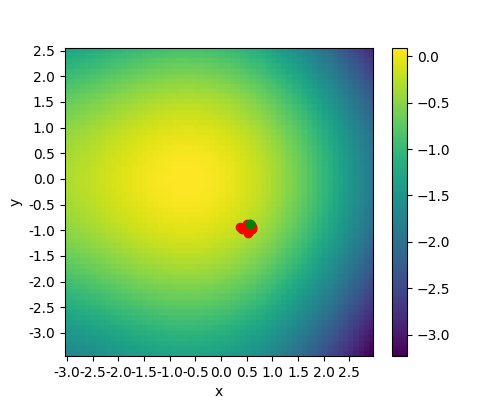
\includegraphics[width=\linewidth]{p7_v_t368.png}
 		 \caption{Paso 350 de $g(x,y)$.}
 		\label{levelplot}
 	\end{subfigure}
 	\caption{Gráficas de la función para encontrar el maximo local de $g(x,y)$.}  	
\label{graficas}
 \end{figure}
 
\section{Conclusiones} 

A mayores pasos mayor es la cantidad de puntos que encuentren el máximo local de la función, la idea es no tener demasiados pasos para tener un código más eficiente, en la figura \ref{con} tenemos 5 pasos y encuentra el punto máximo local de esta forma es más eficaz. Para la resolución de problemas dende es necesario hallar un máximo o un mínimo local en el experimento que el método llega al máximo local.


\begin{figure} [h!]
 	\centering
 	\begin{subfigure}[b]{0.45\linewidth}
 		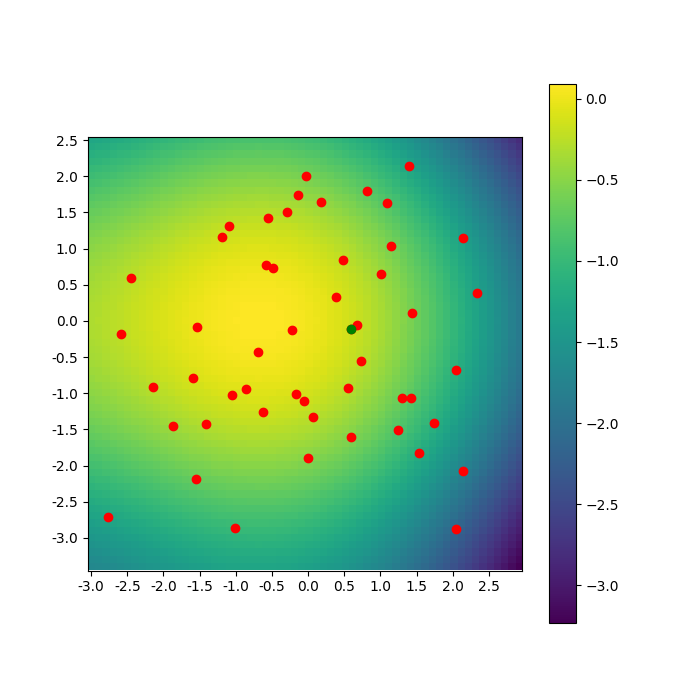
\includegraphics[width=\linewidth]{p7_v_t005.png}
 		 \caption{Paso 1 $g(x,y)$.}
 		\label{3d}
 	\end{subfigure}
 	\begin{subfigure}[b]{0.45\linewidth}
 		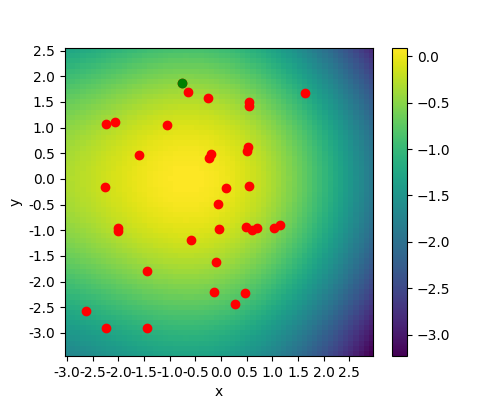
\includegraphics[width=\linewidth]{p7_v_t04.png}
 		 \caption{Paso 5 $g(x,y)$.}
 		\label{levelplot}
 	\end{subfigure}
 	\caption{Gráficas de conclucion la función $g(x,y)$.}
 	\label{con}
 \end{figure}

\bibliography{bib}
\bibliographystyle{plainnat}

\end{document}